
\chapter{Writing \LaTeX}

This is the start of a chapter and gives some introduction before its first section.  This chapter describes basic \LaTeX you need to know.

\section{Sectioning}

The following sectioning macros are available, ordered in descending
importance:

\begin{verbatim}
\chapter{A Chapter}
\section{A Section}
\subsection{A Sub Section}
\subsubsection{A Sub Sub Section}
\subsubsubsection{A Sub Sub Sub Section}
\subsubsubsubsection{A Sub Sub Sub Sub Section}
\end{verbatim}

Starting from \verb|\subsection|, this produces the following:

\subsection{A Sub Section}
\subsubsection{A Sub Sub Section}
\subsubsubsection{A Sub Sub Sub Section}
\subsubsubsubsection{A Sub Sub Sub Sub Section}

Just after defining a chapter and any significant section a
\verb|\label| should be added so it can be referenced.  For example:

\begin{verbatim}
\chapter{A Chapter}
\label{ch:a-chapter}

\section{A Section}
\label{sec:a-section}

\subsection{A Sub Section}
\label{subsec:an-important-sub-section}
\end{verbatim}

See section~\ref{sec:refs} for more on how to reference sections.


\section{Figures}
\label{sec:figures}

See Section~\ref{sec:figures} for guidelines on the graphics files themselves.
Any graphics element is included using this command:

\begin{verbatim}
\includegraphics[OPTIONS]{myfigurefile}
\end{verbatim}

The file's extension may be optionally omitted.
The file is located relative to the directories given in the guidance in Section~\ref{sec:files}.  If a path is given is should be relative to the top-level directory.
The \texttt{OPTIONS} most likely used will be to scale the graphic to
a sensible size.  Examples:

\begin{verbatim}
\includegraphics[width=0.5\textwidth]{...}
\includegraphics[height=0.1\textheight]{...}
\end{verbatim}

Graphics should always be placed in \texttt{figure} environments and include reference label (see
section~\ref{sec:refs} for how to reference figures and tables) and a
caption.  Captions will be printed in the ``List of Figures''.  A
synopsis of a caption should be given in ``[]'' in order to make the
entries in the List of Figures brief and readable.  

Here is an example of adding a figure:
%  http://www-visualmedia.fnal.gov/VMS_Site/gallery/stillphotos/2007/0300/07-0329-14D.jpg
\begin{verbatim}
\begin{figure}[h]
  \centering
  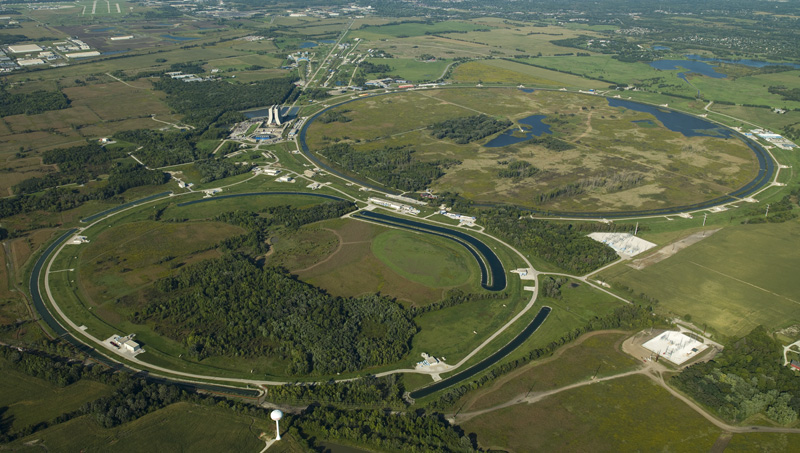
\includegraphics[width=\textwidth]{fermilab-aerial.jpg}
  \caption[Aerial Photo of Fermilab]{An aerial photograph of Fermilab
    showing Wilson Hall and surrounding accelerator rings (Fermilab
    Visual Media Services).}
  \label{fig:fermilab-aerial}
\end{figure}
\end{verbatim}

\begin{figure}[h]
  \centering
  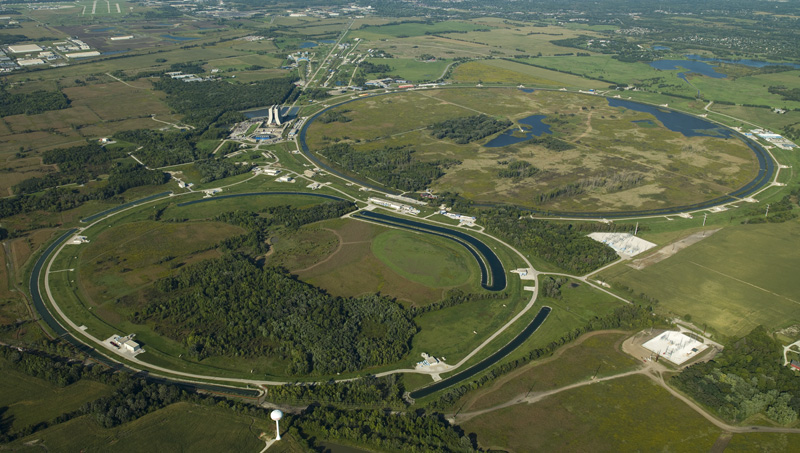
\includegraphics[width=\textwidth]{fermilab-aerial.jpg}
  \caption[Aerial Photo of Fermilab]{An aerial photograph of Fermilab
    showing Wilson Hall and surrounding accelerator rings (Fermilab
    Visual Media Services).}
  \label{fig:fermilab-aerial}
\end{figure}

\section{Tables}
\label{sec:tables}

Tables (actually ``tabular'' environments in a table floating environment) are defined like:

\begin{verbatim}
\begin{table}[h]
  \centering
  \begin{tabular}[h]{|r|c|l|}
    \hline
    Column1 & Column2 & Column3 \\
    \hline
    thing1 & thing2 & thing 3 \\
    \hline
  \end{tabular}
  \caption[Table of things]{A table showing some things}
  \label{tab:things}
\end{table}
\end{verbatim}
\begin{table}[h]
  \centering
  \begin{tabular}[h]{|r|c|l|}
    \hline
    Column1 & Column2 & Column3 \\
    \hline
    thing1 & thing2 & thing 3 \\
    \hline
  \end{tabular}
  \caption[Table of things]{A table showing some things}
  \label{tab:things}
\end{table}

\section{Referencing}
\label{sec:refs}
Note: if you see a ``\textbf{LABEL: ``sec:refs''}'' just above this
line (or elsewhere in chapters, sections, figures, etc), it means this
document was built in draft mode.  This is to help you know what label
to use to reference things.

After any chapter, section or important sub- (subsub-, etc) section or
within any figure or table environment that may need to be referenced
elsewhere in the text one should define a label (\verb|label{...}|).
The defined label can then be used in a \verb|\ref{...}| in order to
make reference to the chapter, section, figure, etc.  For example:

\begin{verbatim}
\chapter{Some Chapter}
\label{ch:some-chapter}

\subsection{Some Sub Section}
\label{subsec:some-sub-section}

...

As described in chapter~\ref{ch:some-chapter} ...

As shown in Figure~\ref{fig:large-cavity} ...
\end{verbatim}

Examples for figures and tables have been given above.  Here I
reference this section:~\ref{sec:refs}.  

